\subsection{Valutazione dell'usabilità (a priori)}

    \begin{flushleft}
       Per la valutazione dell'usabilità del nostro applicativo a priori, cioè prima della fase di sviluppo vera a propria,
       abbiamo deciso di imporci come linee guida le euristiche di Nielsen.
       Ne sono 10, ma vorremmo richiamare l'attenzione su alcune di esse nello specifico:
        \begin{itemize}
            \item  \emph{1. Visibilità dello stato del sistema.} Il sistema presentava una discreta mancanza di feedback, che prevediamo di colmare con elementi quali Dialog, Toast, AlertDialog e SnackBar.
            \item  \emph{2. Corrispondenza fra il mondo reale e il sistema.} Il sistema parla il linguaggio dell' utente utilizzatore del sistema. Tutto ciò che è inerente alle attività di ristorazione è riportato 1:1 in-app.
            \item  \emph{3. Libertà e controllo da parte degli utenti.} In questo tipo di applicazione è raro che l'utente abbia bisogno di tasti undo e redo. In ogni caso, per funzioni complesse, saranno presenti dialog di conferma per eventualmente annullare determinate azioni.
            \item  \emph{4. Consistenza e standard.} Ogni azione è ben contraddistinta da icone, segni, e flow che richiamano esattamente ciò che deve fare. 
            \item  \emph{5. Flessibilità ed efficienza d’uso} Riteniamo che il sistema da costruire non sia particolarmente difficile da gestire. Inoltre, le azioni sono sempre semplici e ben definite.
            \item  \emph{6. Design minimalista ed estetico.} All'inizio abbiamo notato un design antiestetico ma semplcie. Sarà affinato successivamente.
            \item  \emph{7. Prevenzione degli errori.} Il sistema reagisce in maniera controllata e predeterminata alle situazioni di errori che gli utenti possono causare. Nulla è lasciato al caso, ed è, nelle build provate dal team, gestita qualsiasi azione eseguibile dagli utenti.
            \item  \emph{8. Riconoscere piuttosto che ricordare.} La nostra app è dotata di sezioni ben distinte, interfacce dinamiche a seconda del tipo di utente che le usa, e icone e testi ecplicativi dell'azione che si va a intrapendere.
            \item \emph{9.Aiutare gli utenti a riconoscere gli errori, diagnosticarli e correggerli} Sono svariati i feedback sui campi di testo, i Toast, e i dialog se si cercano di compiere azioni illegali. Verrano poi migliorati.
            \item  \emph{10. Guida e documentazione.} E' presente un simpatico topolino (che richiama il logo dell'app) che consiglia tramite vignette e piccoli dialoghi le azioni che si possono intraprendere. Inoltre ci sono piccole note che segnalano campi obbligatori e altri limiti.\\
            Riteniamo che l'applicazione non necessiti un "manuale d'uso", in quanto, come già detto, è minimale e semplice da utilizzare.
        \end{itemize}
    \end{flushleft}

    \begin{figure}[H]
        \centering
        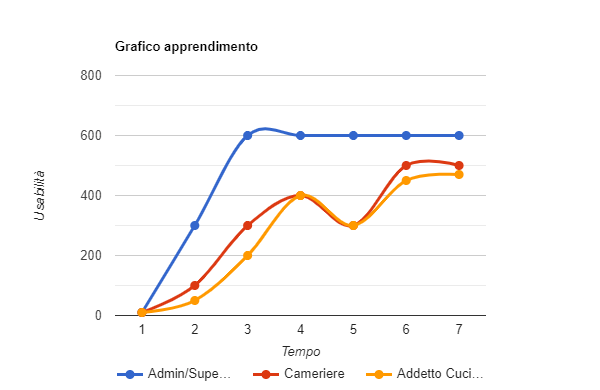
\includegraphics[scale=0.6]{assets/immagini varie/grafico usabilita.png}
        \caption{\textbf{Grafico}: Usabilità}\label{fig:Usabilità_graph}
    \end{figure}
    \vspace{0.5cm}
    \subsubsection*{Considerazioni sull'usabilita}
        \begin{flushleft}
            Riteniamo, in base ad una prima analisi, che quelli che faranno più fatica ad apprendere il funzionamento dell'app potrebbero essere inizialmente admin e supervisori.
            Questo perchè, sono, nella nostra "gerarchia" di funzionalità, quelli che ne posseggono di più. 
            Ma come possiamo notare, sono anche quelli capaci di mantenere costante il grado di conoscenza dell'applicativo.
            Camerieri e addetti alla cucina, in base anche ai turni svolti nel ristorante, alle fasce di punta più affolatte, potrebbero talvolta
            soffrire di rallentamente grafici, di bug, e di layout ancora non troppo ottimizzati per gestire grandi quantità di ordini.
            Inoltre sono il tipo di personale che più velocemente cambia in un ristorante, dovendo cosi riniziare il ciclo di apprendimento.
        \end{flushleft}